\documentclass[10pt,conference]{IEEEtran}
\IEEEoverridecommandlockouts

\usepackage{cite}
\usepackage{amsmath,amssymb,amsfonts}
\usepackage{algorithmic}
\usepackage{graphicx}
\usepackage{textcomp}
\usepackage{xcolor}
\usepackage{url}
\usepackage{booktabs}
\usepackage{float}
\usepackage{newtxtext,newtxmath}
\usepackage{courier}
\usepackage[letterpaper, top=0.88in, bottom=1.05in, left=0.68in, right=0.68in]{geometry}

\setlength{\columnsep}{0.27in}

\makeatletter
\renewcommand{\normalsize}{%
   \@setfontsize\normalsize{11.5}{14}%
   \abovedisplayskip 10\p@ \@plus2\p@ \@minus5\p@
   \abovedisplayshortskip \z@ \@plus3\p@
   \belowdisplayshortskip 6\p@ \@plus3\p@ \@minus3\p@
   \belowdisplayskip \abovedisplayskip
   \let\@listi\@listI}
\normalsize
\makeatother

\title{An Open IEC 62443 Assessment Framework for Manufacturing IACS: Design and Empirical Case Study}

\author{
\IEEEauthorblockN{Yashwanth Sai Tirukkovalluru}
\IEEEauthorblockA{\textit{California State University Channel Islands} \\
Email: yashwanthsai.tirukkovalluru058@myci.csuci.edu}
}

\begin{document}
\pagestyle{plain}

\maketitle

\begin{abstract}
Industrial Automation and Control Systems (IACS) in manufacturing environments face escalating cyber threats while operational constraints limit the application of conventional IT security controls. The IEC 62443 standard family provides comprehensive guidance for IACS security, including Security Level (SL) targets, zones and conduits, and security management systems; however, practitioners lack integrated, reproducible tools that combine compliance assessment with risk-based prioritization. This paper presents the design and implementation of an open-source web assessment platform that operationalizes IEC 62443 through four modules: a 107-item compliance checklist mapped to standard parts 1-4, an SL-Target calculator based on the IEC threat actor model, a zones-and-conduits planner aligned with IEC 62443-3-2, and a five-by-five risk register. We validate the artifact through a pilot case study using a structured representative manufacturing scenario developed at California State University Channel Islands. Results show 49.1\% overall compliance maturity, with System requirements lowest (43.6\%) and two of five architectural zones exhibiting SL-Achieved below SL-Target (DMZ and Operations). Ten risks were registered, including four critical items (risk score at least 15) related to vendor remote access, unpatched PLCs, and MES-OT integration. The study demonstrates that integrated SL-gap and risk analysis surfaces remediation priorities not evident from compliance percentage alone. The artifact, dataset pipeline, and export formats support reproducible OT security research and practitioner baseline assessments.
\end{abstract}

\begin{IEEEkeywords}
IEC 62443, IACS, industrial cybersecurity, operational technology, security level, SCADA, risk assessment
\end{IEEEkeywords}

\section{Introduction}
\IEEEPARstart{M}{anufacturing} organizations increasingly interconnect programmable logic controllers (PLCs), human-machine interfaces (HMIs), manufacturing execution systems (MES), and enterprise IT through Industry~4.0 architectures. This convergence expands the attack surface of Operational Technology (OT) while preserving stringent requirements for availability, safety, and deterministic control---constraints that distinguish IACS security from enterprise information security~\cite{stouffer2023nist825}.

The IEC~62443 standard series, developed by ISA99 and adopted internationally, defines terminology, security management systems (62443-2-1), system requirements including zones and conduits (62443-3-2), and component requirements (62443-4-2). Despite widespread reference in regulatory and customer security questionnaires, organizations report difficulty translating normative requirements into repeatable on-site assessments. Common practice relies on spreadsheets, consultant-led audits, or IT-centric Governance, Risk, and Compliance (GRC) platforms that lack native Security Level semantics and OT-specific risk workflows.

\textbf{Research gap.} Prior academic studies analyze IEC~62443 applicability in energy and IIoT contexts~\cite{vtt2018industrial}, yet few publish open, integrated artifacts combining compliance checklists, SL-Target determination, zone modeling, and exportable audit evidence suitable for research replication.

\textbf{Contributions.} This paper makes four contributions:
\begin{enumerate}
    \item An open-source assessment platform integrating compliance, SL-T, zones/conduits, and risk registration aligned with IEC~62443-3-2.
    \item A reproducible pipeline mapping 107 assessment questions from a structured compliance matrix to machine-readable JSON.
    \item Empirical baseline results from a pilot manufacturing scenario: 49.1\% maturity, SL gaps, and four critical risks.
    \item Evidence that integrated assessment prioritizes remediation beyond checklist scores alone.
\end{enumerate}

\section{Related Work}
\textbf{IACS security frameworks.} NIST SP~800-82 Rev.~3~\cite{stouffer2023nist825} provides ICS-specific security guidance but does not define SL-T or zones/conduits using IEC semantics. ISO/IEC~27019 addresses process control in IT-dependent environments but complements rather than replaces 62443 for OT components.

\textbf{IEC~62443 application.} Practitioner literature from SANS and ISA99 introduces program-level implementation~\cite{isa99intro}. Academic work includes IIoT vulnerability assessment mapped to 62443 and energy-sector case analyses. VTT technical reports document industrial cyber risk in Nordic critical infrastructure~\cite{vtt2018industrial}. These sources establish theoretical grounding but rarely ship maintainable assessment tools.

\textbf{OT security tools.} Commercial platforms (e.g., Claroty, Dragos, Nozomi) emphasize asset discovery and anomaly detection. Our artifact complements such tools by addressing \emph{normative} IEC~62443 compliance mapping and structured audit export---a reproducibility niche for researchers and OT security engineers establishing IACS Security Management Systems.

\section{Methodology}
We adopt Design Science Research (DSR)~\cite{hevner2004design}: (1)~problem identification, (2)~artifact design, (3)~demonstration, (4)~evaluation, (5)~communication. Evaluation combines descriptive metrics from a \emph{pilot} case study using a structured representative manufacturing scenario developed during a university research project at California State University Channel Islands.

\textbf{Structured pilot scenario.} The case study is \emph{not} an on-site plant audit or hardware-in-the-loop test. Instead, we define a reference architecture (Purdue-style zones, representative assets, conduits) and a reproducible JSON dataset (\texttt{sample-assessment.json}) containing 107 compliance responses, five zone records, and ten risk entries. A Python script seeds brownfield-like answer distributions; zones and risks were authored from common OT weakness patterns in the literature. The open-source tool computes all reported metrics from this input---demonstrating the assessment pipeline rather than validating live operational telemetry.

\textbf{System Under Consideration (SuC).} The SuC models a representative assembly line with four Siemens S7-1500 PLCs, HMIs, engineering workstations, PI historian connectivity, MES integration, and vendor remote access via a DMZ jump host---consistent with published brownfield manufacturing OT architectures.

\textbf{Compliance maturity.} For $n$ assessed questions, maturity is:
\begin{equation}
M = \frac{Y + 0.5P}{n} \times 100
\end{equation}
where $Y$ counts ``Yes'' responses, $P$ counts ``Partial,'' excluding N/A.

\textbf{Risk score.} Each risk receives likelihood $L$ and impact $I$ on $[1,5]$; $R = L \times I$. Critical risks satisfy $R \geq 15$.

\textbf{SL gap.} For each zone, $\Delta SL = SL\text{-}T - SL\text{-}A$; positive gap indicates remediation need per IEC~62443-3-2 verification guidance.

\section{Artifact Design}
The platform comprises four browser-based modules backed by local storage (no cloud upload of sensitive OT data):

\textbf{Compliance module.} One hundred seven questions extracted from a structured Excel matrix cover General, Policies and Procedures, System, and Component parts. Responses support Yes/Partial/No/N/A with evidence notes.

\textbf{SL calculator.} Threat characteristics (misuse type, means, resources, knowledge, motivation) map to recommended SL-T (0--4) following IEC~62443-3-2/3-3 threat models.

\textbf{Zones and conduits.} Users define zones with SL-T and SL-A; a Purdue reference template accelerates modeling.

\textbf{Risk register.} Risks link to zones; a heat map visualizes $L \times I$ distribution.

\textbf{Deployment.} Static build (React/Vite) deploys via Docker/nginx or GitHub Pages. Python scripts regenerate JSON from the source Excel matrix.

\textbf{Architecture.} Fig.~\ref{fig:architecture} shows the zones-and-conduits module with SL-T/SL-A comparison for the pilot scenario. All assessment data remain in browser \texttt{localStorage} unless the user exports JSON/CSV; no OT configuration data are transmitted to external services---supporting air-gapped engineering use.

\begin{figure}[!t]
\centering
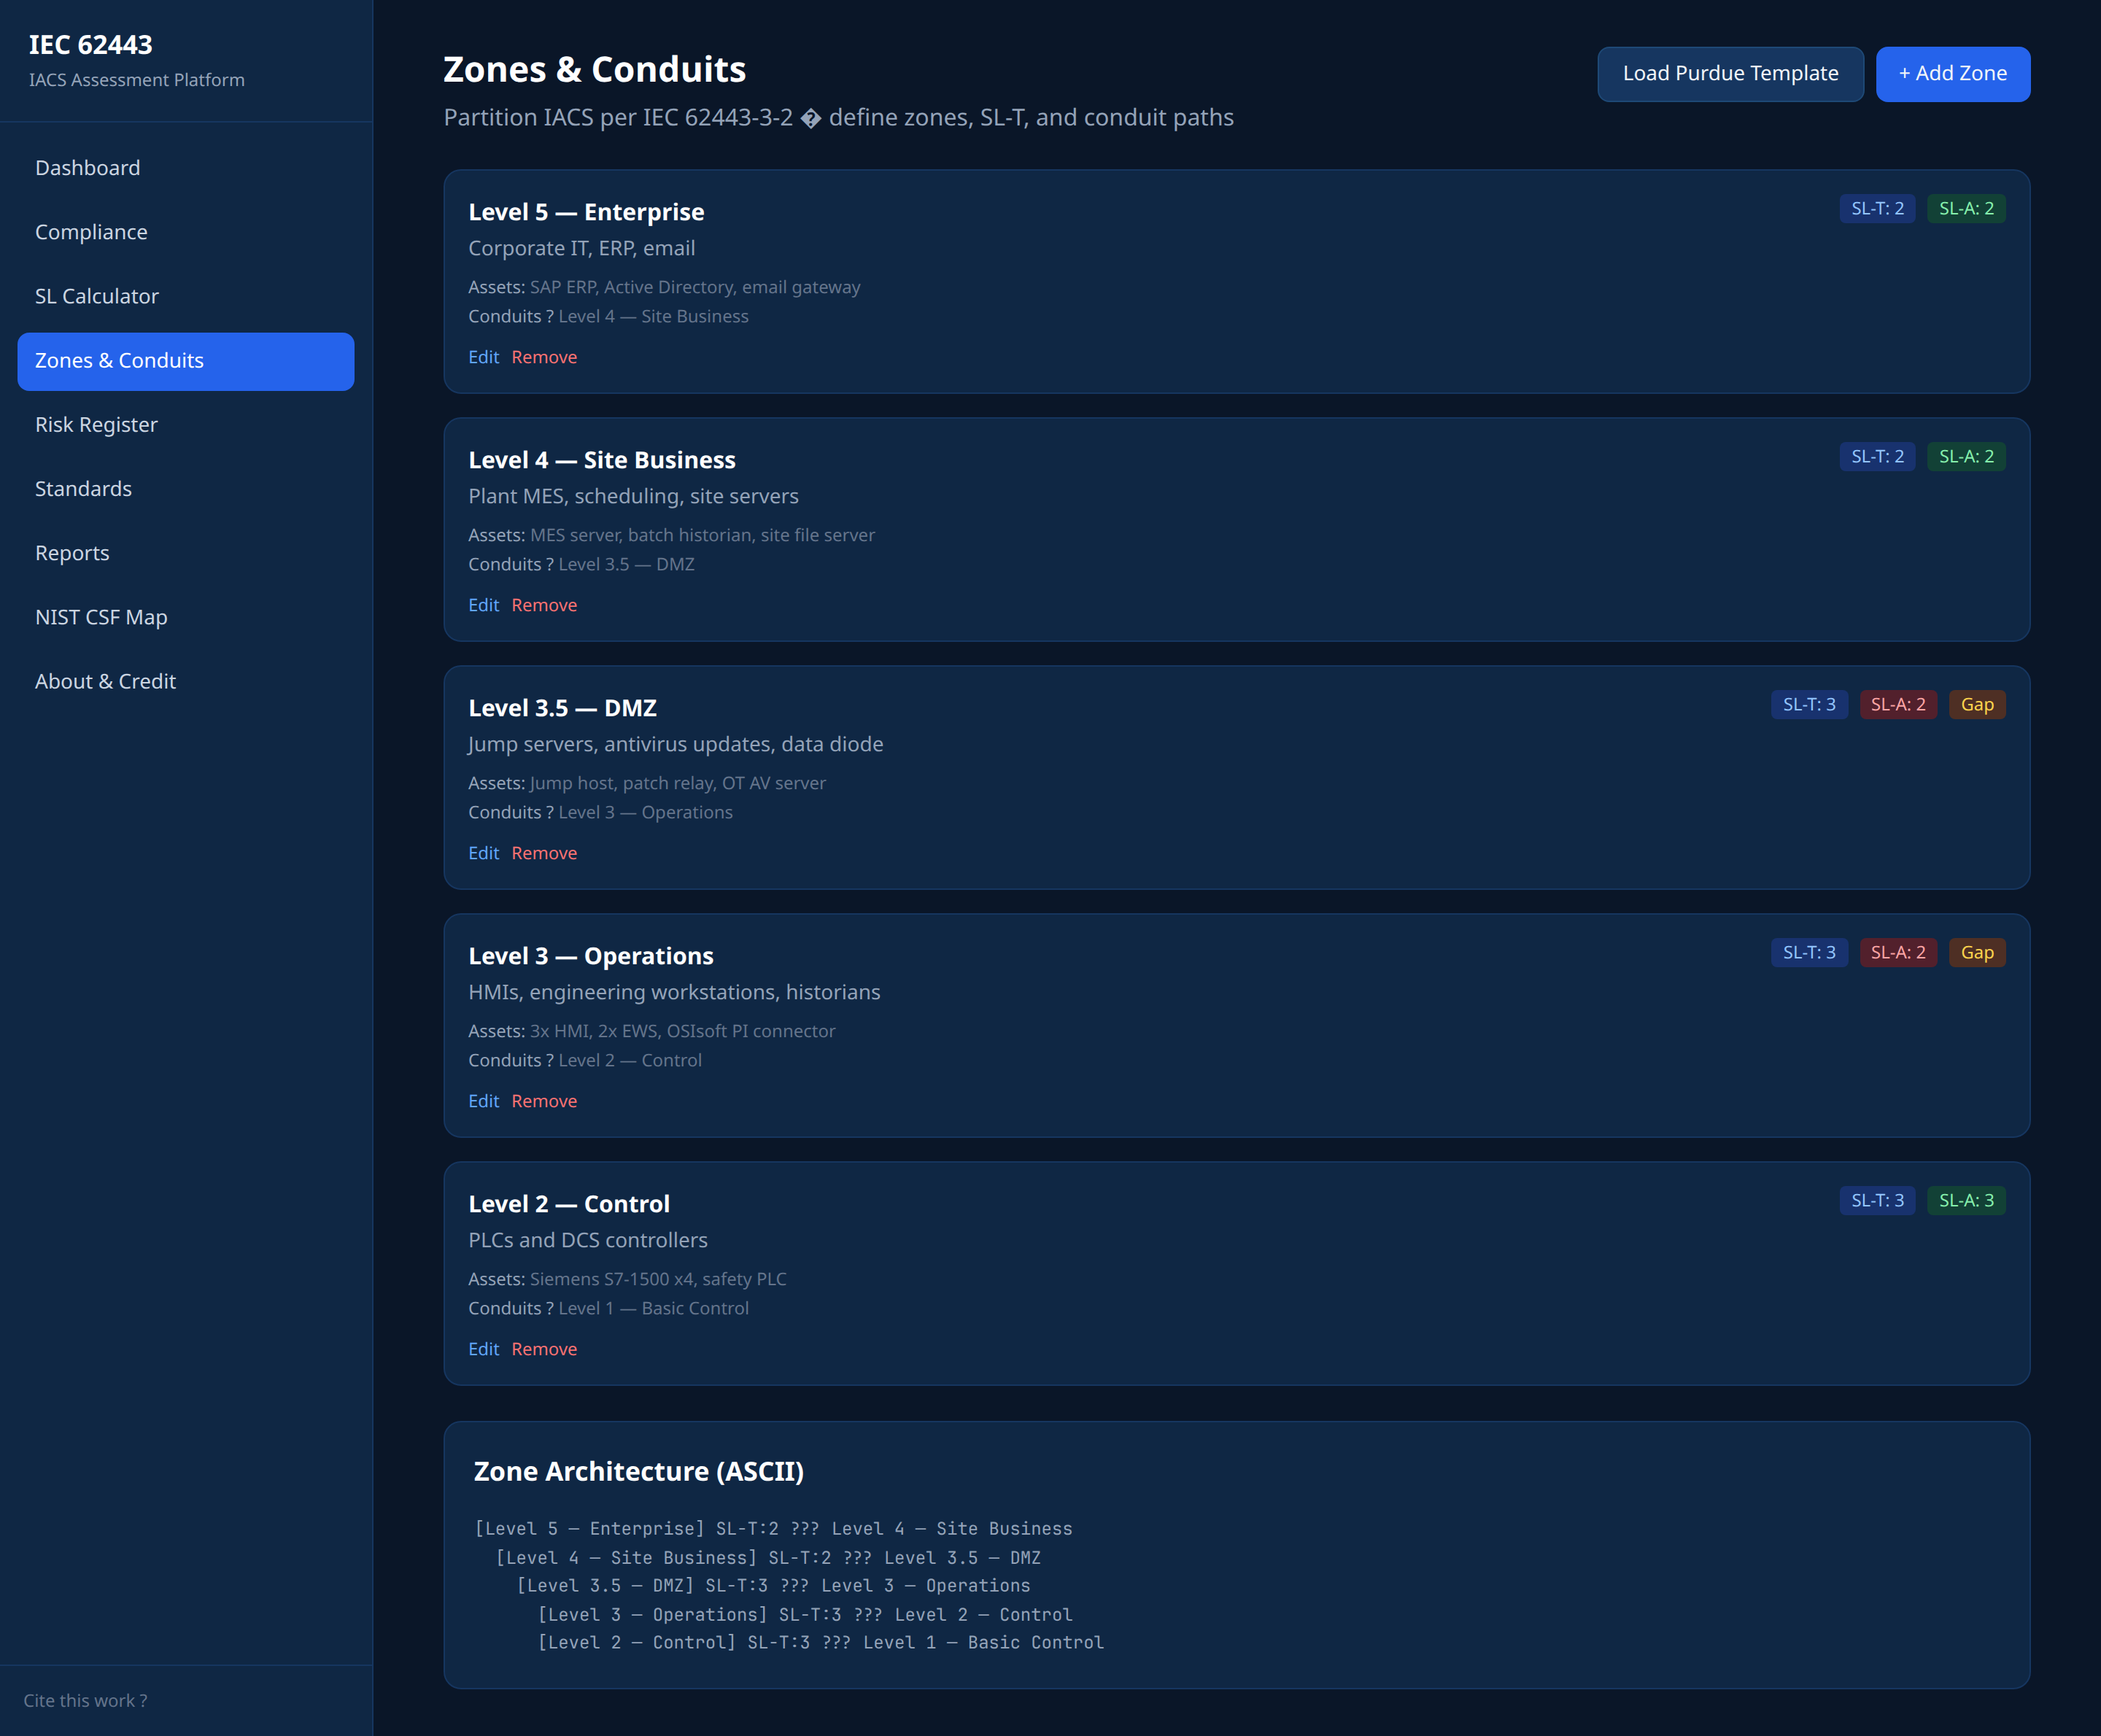
\includegraphics[width=\linewidth]{figures/zones-screenshot.png}
\caption{Zones and conduits view with SL-T/SL-A gaps (pilot scenario). Live demo: GitHub Pages deployment.}
\label{fig:architecture}
\end{figure}

\textbf{Reproducibility pipeline.} (1)~Excel compliance matrix $\rightarrow$ \texttt{extract\_requirements.py} $\rightarrow$ \texttt{iec62443.json}; (2)~optional \texttt{generate\_sample\_case\_study.py} $\rightarrow$ pilot dataset; (3)~web app load $\rightarrow$ dashboard metrics; (4)~export JSON/CSV for audit evidence. This pipeline supports thesis replication and practitioner baseline assessments without vendor lock-in.

\section{Case Study Results}
\subsection{Compliance Maturity}
Overall maturity was \textbf{49.1\%}. By standard part: General 66.7\%, Policies and Procedures 55.0\%, System 43.6\%, Component 53.4\%. System requirements---including monitoring, segmentation verification, and SL-A documentation---showed the largest gap, consistent with brownfield sites lacking dedicated OT security staff.

\begin{figure}[H]
\centering
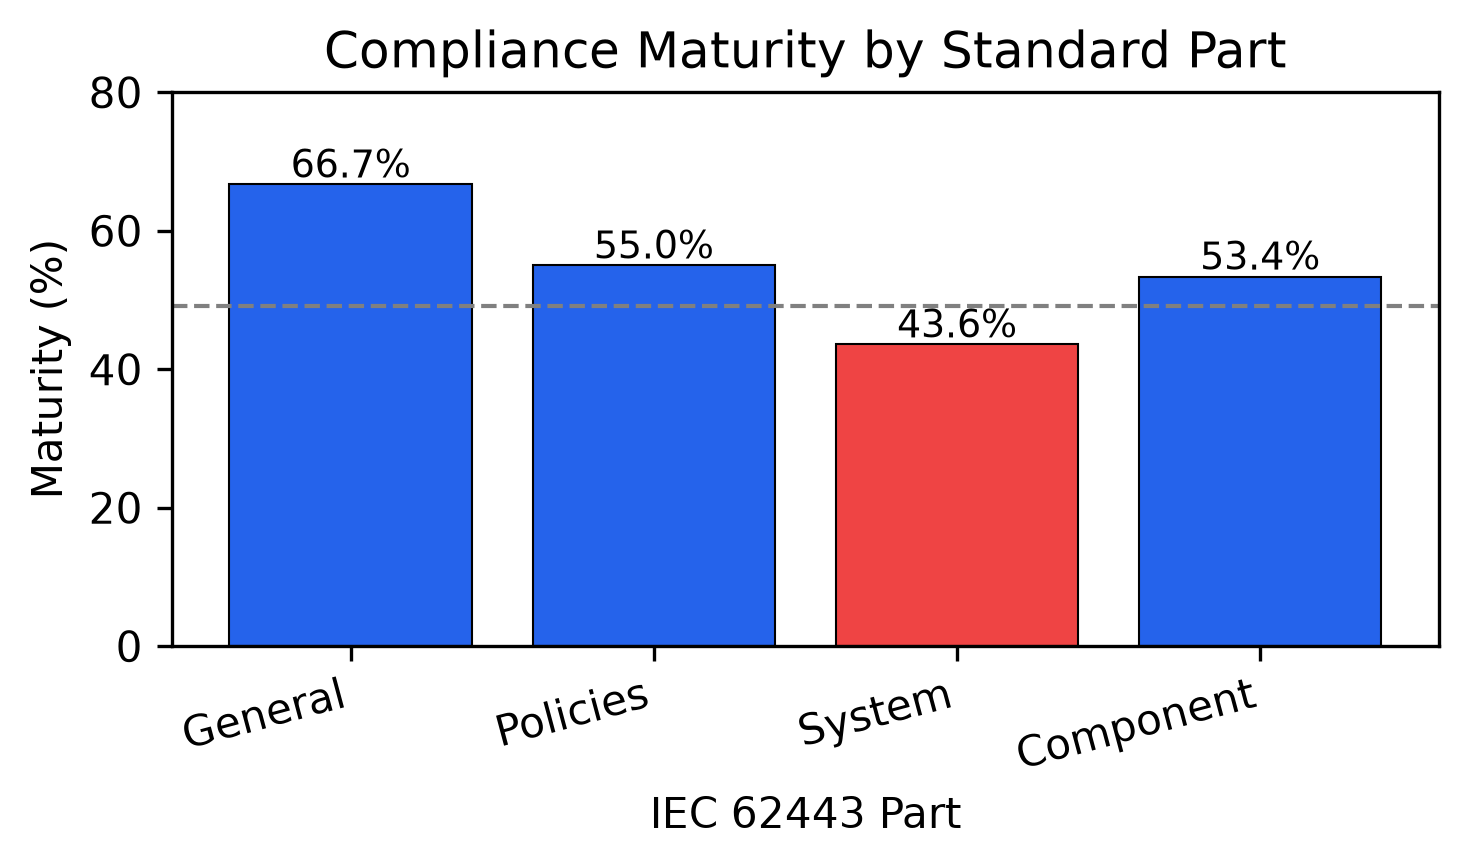
\includegraphics[width=\linewidth]{figures/maturity-by-part.png}
\caption{Compliance maturity by IEC 62443 part (pilot scenario, $n=107$ questions).}
\label{fig:maturity}
\end{figure}

\subsection{Security Level Analysis}
Five zones were modeled (Enterprise through Control). Table~\ref{tab:zones} summarizes SL-T, SL-Achieved, and $\Delta$SL. Two zones exhibited gaps ($\Delta$SL $= 1$): DMZ (vendor jump host, patch relay) and Operations (HMIs, engineering workstations, historian). Control achieved SL-A=3 matching SL-T=3; Enterprise zones met SL-T=2.

\begin{table}[!t]
\caption{Zone Security Levels (Purdue Reference Model)}
\label{tab:zones}
\centering
\small
\begin{tabular}{lccc}
\hline
Zone & SL-T & SL-A & $\Delta$SL \\
\hline
L5 Enterprise & 2 & 2 & 0 \\
L4 Site Business & 2 & 2 & 0 \\
L3.5 DMZ & 3 & 2 & 1 \\
L3 Operations & 3 & 2 & 1 \\
L2 Control (4$\times$ S7-1500) & 3 & 3 & 0 \\
\hline
\end{tabular}
\end{table}

\subsection{Risk Register}
Ten risks were identified; eight remain open. Table~\ref{tab:risks} lists critical items ($R \geq 15$). Vendor remote access scored highest ($R=20$) despite moderate System-part compliance---illustrating why integrated risk scoring complements checklist maturity.

\begin{table}[!t]
\caption{Critical Risks ($R \geq 15$) from Pilot Scenario}
\label{tab:risks}
\centering
\small
\begin{tabular}{p{0.22\linewidth}cccp{0.18\linewidth}}
\hline
Asset & $L$ & $I$ & $R$ & Zone \\
\hline
Vendor jump server & 4 & 5 & 20 & DMZ \\
Engineering WS (USB) & 4 & 4 & 16 & Operations \\
S7-1500 PLCs & 3 & 5 & 15 & Control \\
MES--OT integration & 3 & 5 & 15 & Site Business \\
\hline
\end{tabular}
\end{table}

\subsection{Integrated Findings}
Compliance maturity alone would emphasize System-part controls (43.6\%) but not prioritize vendor access (DMZ) as the highest risk score. Integrated analysis recommends: (1)~MFA on jump servers within 90 days; (2)~OT patch program per 62443-2-3; (3)~MES--OT conduit hardening within 12 months.

\begin{table}[!t]
\caption{Compliance Maturity by IEC 62443 Part}
\label{tab:maturity}
\centering
\begin{tabular}{lrr}
\hline
Part & Maturity (\%) & $n$ \\
\hline
General & 66.7 & 3 \\
Policies \& Procedures & 55.0 & 20 \\
System & 43.6 & 55 \\
Component & 53.4 & 29 \\
\hline
\textbf{Overall} & \textbf{49.1} & \textbf{107} \\
\hline
\end{tabular}
\end{table}

\section{Discussion}
Results align with practitioner reports: manufacturing sites initiate IEC~62443 program documentation (Policies 55\%) before completing technical SL verification (System 43.6\%). SL gaps concentrate at IT/OT integration boundaries---a finding consistent with 62443-3-2 conduit emphasis.

\textbf{Limitations.} Four limitations bound generalizability: (1)~structured pilot input rather than live plant walk-through; (2)~SL-Achieved values assigned analytically, not verified from device configurations; (3)~107-question subset of the full 62443 corpus; (4)~single assessor, no inter-rater reliability study. These constraints are appropriate for an artifact demonstration paper but require field validation before operational certification claims.

\textbf{Threats to validity.} Construct validity: maturity scoring treats Partial as 0.5 Yes---sensitive to assessor judgment. External validity: one fictional manufacturing scenario may not represent all sectors (e.g., chemical, water). Conclusion validity: integrated prioritization is descriptive; no control group compared against spreadsheet-only assessment.

\textbf{Industry implications.} OT teams can deploy the Docker-packaged tool on engineering networks without external data transfer. Practitioners can replace pilot JSON with site-specific assessor input while retaining the same SL-gap and risk workflows. NIST Cybersecurity Framework cross-mapping in the tool supports communication with IT security stakeholders.

\section{Conclusion and Future Work}
We presented an open IEC~62443 assessment framework validated through a pilot manufacturing IACS scenario. Future work includes multi-site validation with operational facilities, dual-assessor reliability study, automated SL-A verification from configuration exports, and integration with passive OT asset discovery.

\textbf{Data availability.} Source code and case study export: \url{https://github.com/yashwanth123/CyberSecurity-graduate-research-work-}

\section*{Acknowledgment}
The author thanks faculty at California State University Channel Islands for guidance on this research project, and the IEC~62443 and ISA99 community for public guidance materials used in this work.

\bibliographystyle{IEEEtran}
\bibliography{references}

\end{document}
